\documentclass[pdflatex,sn-mathphys-num]{sn-jnl}

\usepackage{graphicx}
\usepackage{xcolor}
\usepackage{multirow}
\usepackage{amsmath,amssymb,amsfonts}
\usepackage{booktabs}
\usepackage{enumitem}
\usepackage{algorithm}
\usepackage{algorithmicx}
\usepackage{algpseudocode}

\begin{document}

\title[DRL for Risk-Adjusted Cryptocurrency Portfolio Management]{Deep Reinforcement Learning for Risk-Adjusted Cryptocurrency Portfolio Management}

\author*[1]{\fnm{Nguyen Trong} \sur{Hieu}}\email{hieuntse183303@fpt.edu.vn}
\author[1]{\fnm{Luu Duc} \sur{Anh}}\email{anhldse183141@fpt.edu.vn}
\author[1]{\fnm{Nguyen Duc} \sur{Hien}}\email{hienndse173053@fpt.edu.vn}

\affil*[1]{\orgdiv{Artificial Intelligence}, \orgname{FPT University},
  \orgaddress{\city{Ho Chi Minh City}, \country{Vietnam}}}

\abstract{Deep reinforcement learning agents trained for portfolio management
frequently achieve strong simulated returns while accumulating transaction costs
that erode real-world profitability. An initial investigation confirmed this
pattern: a Proximal Policy Optimization (PPO) agent applied to cryptocurrency
assets rebalanced without restraint, accumulating transaction fees that
routinely exceeded the agent's actual alpha. This work addresses the problem through a
three-component framework. First, a price-drift-adjusted no-trade zone suppresses
rebalancing unless the deviation between target and naturally drifted weights
exceeds a threshold of 5\%. Second, a cash allocation slot is incorporated as a
learnable defensive position, allowing the agent to reduce market exposure without
any hard-coded exit rule. Third, a quadratic drawdown penalty escalates as losses
deepen, creating a strong incentive to seek capital preservation under adverse
conditions. Evaluated on BTC, ETH, and BNB from 2020 to 2024 using walk-forward
validation, the proposed system reduced annual transaction costs below 0.6\%
while maintaining competitive risk-adjusted performance. Systematic experiments
across three reward formulations, two network architectures, and three random
seeds confirm the reproducibility of these findings.}

\keywords{deep reinforcement learning, portfolio management, cryptocurrency,
Proximal Policy Optimization, transaction costs, no-trade zone}

\maketitle

%%=============================================================%%
\section{Introduction}\label{sec:introduction}
%%=============================================================%%

Cryptocurrency markets have grown from a niche curiosity into a multi-trillion
dollar asset class over the past decade. This expansion has attracted substantial
research attention in automated trading, where the high volatility and continuous
24/7 operation of crypto markets present challenges that are qualitatively
different from traditional equity environments. BTC can lose 15\% in a single
session. Correlated drawdowns frequently affect multiple assets simultaneously.
Deep reinforcement learning offers a principled approach to this setting: agents
learn allocation strategies directly from market data without requiring explicit
price predictions, and multiple prior studies have demonstrated that RL agents
can outperform naive benchmarks on simulated crypto markets
\cite{jiang2017deep,betancourt2021deep}.

A critical limitation, however, has received insufficient attention in prior work:
transaction costs. Binance charges 0.1\% per trade. Cryptocurrency markets
operate continuously (24/7), and an agent that rebalances without restraint can
accumulate fees that far exceed any realistic alpha. Preliminary experiments in
this study confirmed this pattern directly: an unconstrained PPO agent generated
substantial gross returns but net returns were severely eroded by accumulated
transaction costs.

The root cause is architectural. Conventional RL environments for portfolio
management compare target weights against the \emph{previous day's} weights.
Since prices move continuously, this creates artificial deviations that trigger
unnecessary trades. A concrete example illustrates the issue: a portfolio holds
26\% BTC. Overnight, BTC climbs 1\%, and natural price drift pushes BTC's weight
to 26.2\%. If the agent's new target is 26.3\%, a naive system executes a trade
to close a 0.1\% gap, paying a fee that exceeds any conceivable benefit.
Repeated daily across a full year, the losses are substantial.

This study proposes three complementary interventions. First, a
\textbf{price-drift-adjusted no-trade zone} measures the deviation between
target weights and naturally drifted weights rather than previous-day weights.
Rebalancing occurs only when this deviation exceeds 5\%, eliminating
fee-negative trades while preserving intentional repositioning. Second,
\textbf{cash as a learnable asset} provides an allocation refuge without
any hard-coded market-exit rule; the agent discovers through reward shaping
when capital preservation is preferable to market exposure. Third, a
\textbf{quadratic drawdown penalty} in the reward function creates
progressively stronger incentives to reduce exposure as losses deepen,
mirroring the mathematical asymmetry of drawdown recovery documented in
classical portfolio theory \cite{grossman1993portfolio}.

The specific contributions of this work are:

\begin{enumerate}[leftmargin=*]
\item A \textbf{price-drift adjusted no-trade zone} that substantially reduces annual transaction costs, to below 0.6\% in experiments, without sacrificing risk-adjusted performance.
\item \textbf{Cash as a learned refuge.} The agent autonomously shifts capital into cash under adverse conditions, without any hand-coded exit rule, simply by incorporating cash as a fourth allocation target in the action space.
\item A \textbf{four-component reward function}: log return for growth, downside volatility penalty for risk, turnover penalty to discourage excessive rebalancing, and a quadratic drawdown term that provides escalating incentives for capital preservation.
\item \textbf{Reproducible experiments} across three reward formulations, two network architectures (MLP and LSTM), two training windows, and three random seeds, with both mean and standard deviation reported.
\end{enumerate}

The remainder of this paper is organized as follows. Section~\ref{sec:related}
reviews related work. Section~\ref{sec:data} describes the dataset and
preprocessing procedure. Section~\ref{sec:methodology} presents the full
methodology. Section~\ref{sec:experiments} defines the experimental protocol.
Section~\ref{sec:results} reports and interprets results.
Section~\ref{sec:live} presents a live out-of-sample evaluation covering
March 2025 through March 2026. Section~\ref{sec:limitations} identifies limitations.
Section~\ref{sec:conclusion} concludes.

%%=============================================================%%
\section{Related Work}\label{sec:related}
%%=============================================================%%

\subsection{DRL for Portfolio Management}

The EIIE framework by Jiang et al.\ \cite{jiang2017deep} was among the first
systems to apply neural networks to cryptocurrency asset allocation. Their
architecture combined CNN and RNN layers with a Portfolio-Vector Memory, and
demonstrated that agents could learn effective trading strategies directly from
raw price data. Transaction costs in that work were modeled as a single fixed
rate applied regardless of trade frequency. For agents executing hundreds of
trades per year, this simplification significantly underestimates realized costs.

For equity markets, Yang et al.\ \cite{yang2020deep} proposed an ensemble
approach combining PPO, A2C, and DDPG, switching between algorithms based on
recent Sharpe ratio performance. Liu et al.\ \cite{liu2022finrl} extended this
direction into FinRL, an open-source library providing standardized RL
environments for quantitative finance research. Both contributions focus
primarily on equities; direct application to cryptocurrency markets presents
additional challenges including substantially higher volatility, continuous
trading hours, and periodic liquidity crises in smaller tokens.

\subsection{Risk-Aware Reward Design}

A reward function that maximizes only raw return produces agents that concentrate
positions in recently performing assets, creating portfolios vulnerable to sudden
reversals. Incorporating explicit risk penalties into the reward signal is a
well-established mitigation strategy. Choudhary et al.\ \cite{choudhary2025risk}
systematically compared multiple risk-adjusted reward formulations and found that
explicit risk penalties reliably reduce peak drawdowns, at modest cost to raw
returns. Park et al.\ \cite{park2020risk} embedded Conditional Value-at-Risk
(CVaR) directly into the policy gradient step. The approach in this study
attaches three penalty terms to the reward (downside volatility, turnover, and
quadratic drawdown) and allows the agent to balance them through experience.
This design is both simpler to implement and more interpretable than CVaR
embedding, since each penalty term is directly observable and attributable.

\subsection{Transaction Cost Management}

The divergence between backtest and live performance in RL trading systems is
frequently attributable to inadequate cost modeling. Betancourt and Chen
\cite{betancourt2021deep} developed a DRL system with explicit exchange fee
optimization. Sadighian \cite{sadighian2019deep} demonstrated that backtest
results without realistic cost models systematically overfit to profits that
would not materialize in practice. The approach proposed in this study differs
in emphasis: rather than optimizing execution given that a trade occurs, the
system first determines whether a trade is cost-justified. The no-trade zone
functions as a gating mechanism; a rebalancing action that does not clear the
threshold is suppressed entirely. Betancourt and Chen
\cite{betancourt2021deep} reached a similar empirical finding: once fees are
properly modeled, small weight adjustments contribute negligible net returns.

\subsection{Drawdown Control}

Grossman and Zhou \cite{grossman1993portfolio} established the theoretical
optimality of reducing market exposure as drawdown grows under a hard maximum
drawdown constraint. The intuition is reinforced by the mathematical asymmetry
of recovery: a 10\% loss requires an 11.1\% gain to recover; a 40\% loss
requires a 66.7\% gain. The quadratic drawdown penalty in this study
incorporates this asymmetry as a reward signal, creating progressively stronger
incentives to reduce risk exposure as losses deepen.

%%=============================================================%%
\section{Data}\label{sec:data}
%%=============================================================%%

\subsection{Dataset}

Daily OHLCV data (Open, High, Low, Close, Volume) for Bitcoin (BTC), Ethereum
(ETH), and Binance Coin (BNB) were collected via the Yahoo Finance API, covering
January~1, 2020 through December~31, 2024, producing 1,826 aligned trading days
after cleaning. These three assets were selected on the basis of market
capitalization and order-book depth on Binance.

\subsection{Features}

Six technical indicators per asset, all derived from the closing price series:

\begin{enumerate}[leftmargin=*]
\item \textbf{Close} ($P_t$): the base price series.
\item \textbf{7-day moving average} ($\mathrm{MA7}_t$): short-term trend.
\item \textbf{21-day moving average} ($\mathrm{MA21}_t$): medium-term trend. The MA7/MA21 crossover is a widely observed directional signal.
\item \textbf{RSI, 14-day}: a momentum oscillator bounded to $[0, 100]$. Values above 70 indicate overbought conditions; values below 30 indicate oversold conditions.
\item \textbf{MACD} ($\mathrm{EMA}_{12} - \mathrm{EMA}_{26}$): positive when short-term momentum exceeds long-term momentum.
\item \textbf{14-day realized volatility}: standard deviation of daily log returns over the prior two weeks, providing a direct signal of recent market uncertainty.
\end{enumerate}

\subsection{Normalization}

A rolling z-score with a 60-day lookback is applied to all features:

\begin{equation}\label{eq:zscore}
    z_t = \frac{x_t - \hat{\mu}_{t}}{\hat{\sigma}_{t} + \epsilon}, \quad
    \hat{\mu}_{t} = \frac{1}{60}\sum_{k=1}^{60} x_{t-k}, \quad
    \hat{\sigma}_{t} = \sqrt{\frac{1}{59}\sum_{k=1}^{60}(x_{t-k} - \hat{\mu}_{t})^2}
\end{equation}

The rolling window is essential to prevent look-ahead bias. A global z-score
computed over the entire dataset would embed future statistical information into
early training periods. With a rolling window, all normalization statistics are
derived exclusively from past observations.

\subsection{Data Cleaning}

Days on which any asset moved more than 50\% in a single session were
flagged for review. One such event was identified: BNB on February~19, 2021,
associated with a Binance Smart Chain deployment event rather than genuine
market activity. This observation was removed, and the three time series were
re-aligned by retaining only dates present across all three assets.

\subsection{Walk-Forward Validation}\label{sec:walkforward}

Walk-forward validation replicates the sequential nature of real deployment:
train on historical data, evaluate on the subsequent period, then advance the
training window. Two non-overlapping evaluation periods are used:

\begin{itemize}[leftmargin=*]
\item \textbf{Window 1 (W1)}: Train January 2020--December 2022; Test January--December 2023 (post-bear-market recovery, BTC $+154\%$).
\item \textbf{Window 2 (W2)}: Train January 2021--December 2023; Test January--December 2024 (institutional-driven bull run, BTC $+111\%$).
\end{itemize}

All hyperparameter tuning decisions used W1 exclusively. W2 is a fully
held-out evaluation window; no tuning decisions were informed by its outcomes.

Figure~\ref{fig:walk_forward} illustrates the two training and evaluation windows.

\begin{figure}[htbp]
    \centering
    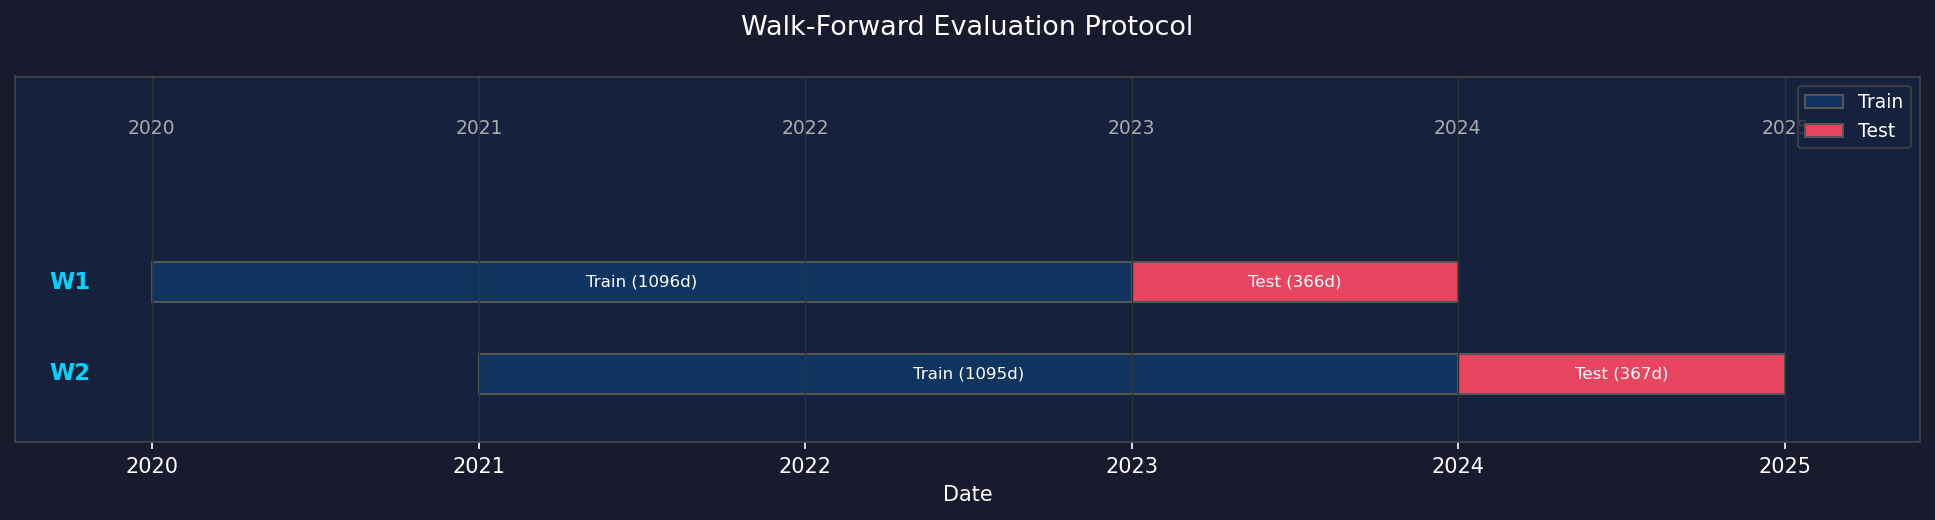
\includegraphics[width=0.9\textwidth]{figures/eda_walk_forward_splits.png}
    \caption{Walk-forward evaluation protocol. Blue regions denote training
    periods; red regions denote held-out test periods. W1 tests on the 2023
    recovery market; W2 tests on the 2024 bull run. The two evaluation windows
    cover qualitatively distinct market regimes, reducing the risk that results
    generalize only to a single regime type.}
    \label{fig:walk_forward}
\end{figure}

\subsection{Exploratory Data Analysis}

Prior to model development, the statistical properties of the three assets were
examined to characterize return distributions and motivate metric selection.

Figure~\ref{fig:return_dist} presents the daily return distributions for all
three assets. All distributions exhibit heavy tails and excess kurtosis (BTC:
11.1, ETH: 8.9, BNB: 34.7), confirming that extreme daily moves occur far
more frequently than a normal distribution would predict. Standard deviation
consequently underestimates true downside risk. This motivates penalizing only
negative deviations (Sortino-style) rather than total variance (Sharpe-style).

\begin{figure}[htbp]
    \centering
    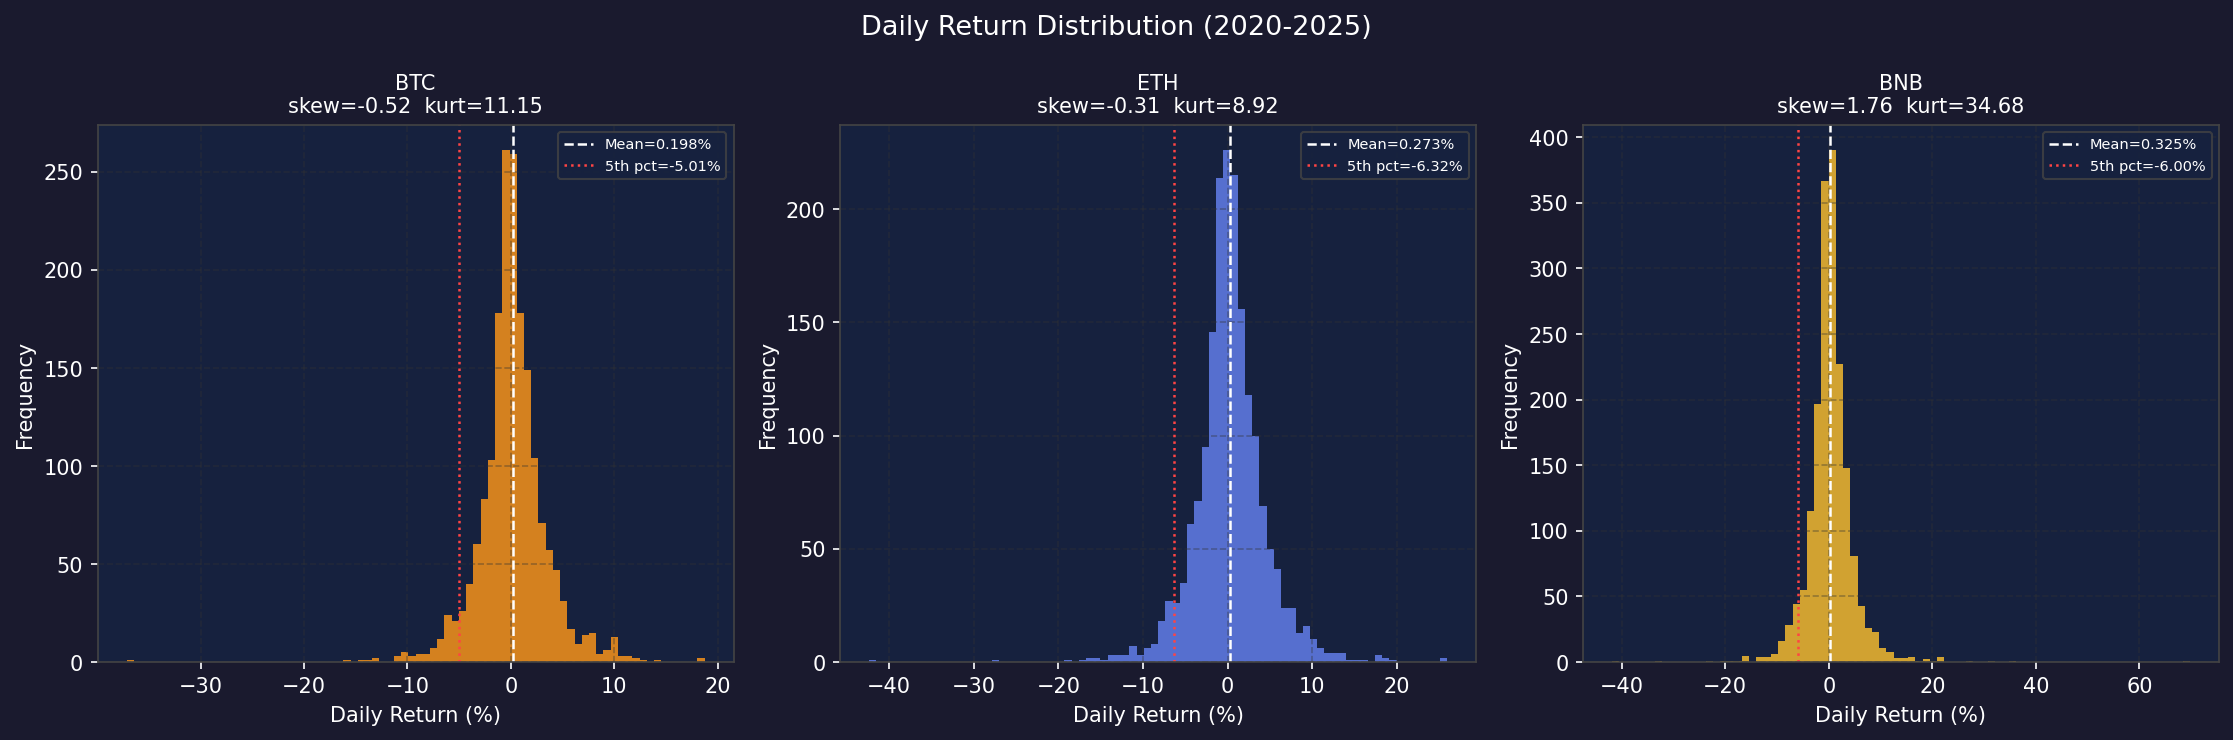
\includegraphics[width=0.9\textwidth]{figures/eda_return_distribution.png}
    \caption{Daily return distributions for BTC, ETH, and BNB (2020--2024).
    All three distributions exhibit heavy tails. BNB's extreme kurtosis (34.7)
    reflects infrequent but very large single-day moves, including the anomalous
    $+69.8\%$ event on 2021-02-19 that was excluded during cleaning.}
    \label{fig:return_dist}
\end{figure}

Figure~\ref{fig:rolling_vol} shows 30-day rolling annualized volatility.
Volatility is clearly time-varying and regime-dependent. The agent observes
14-day realized volatility as one of its six input features, providing a
direct signal of current market conditions.

\begin{figure}[htbp]
    \centering
    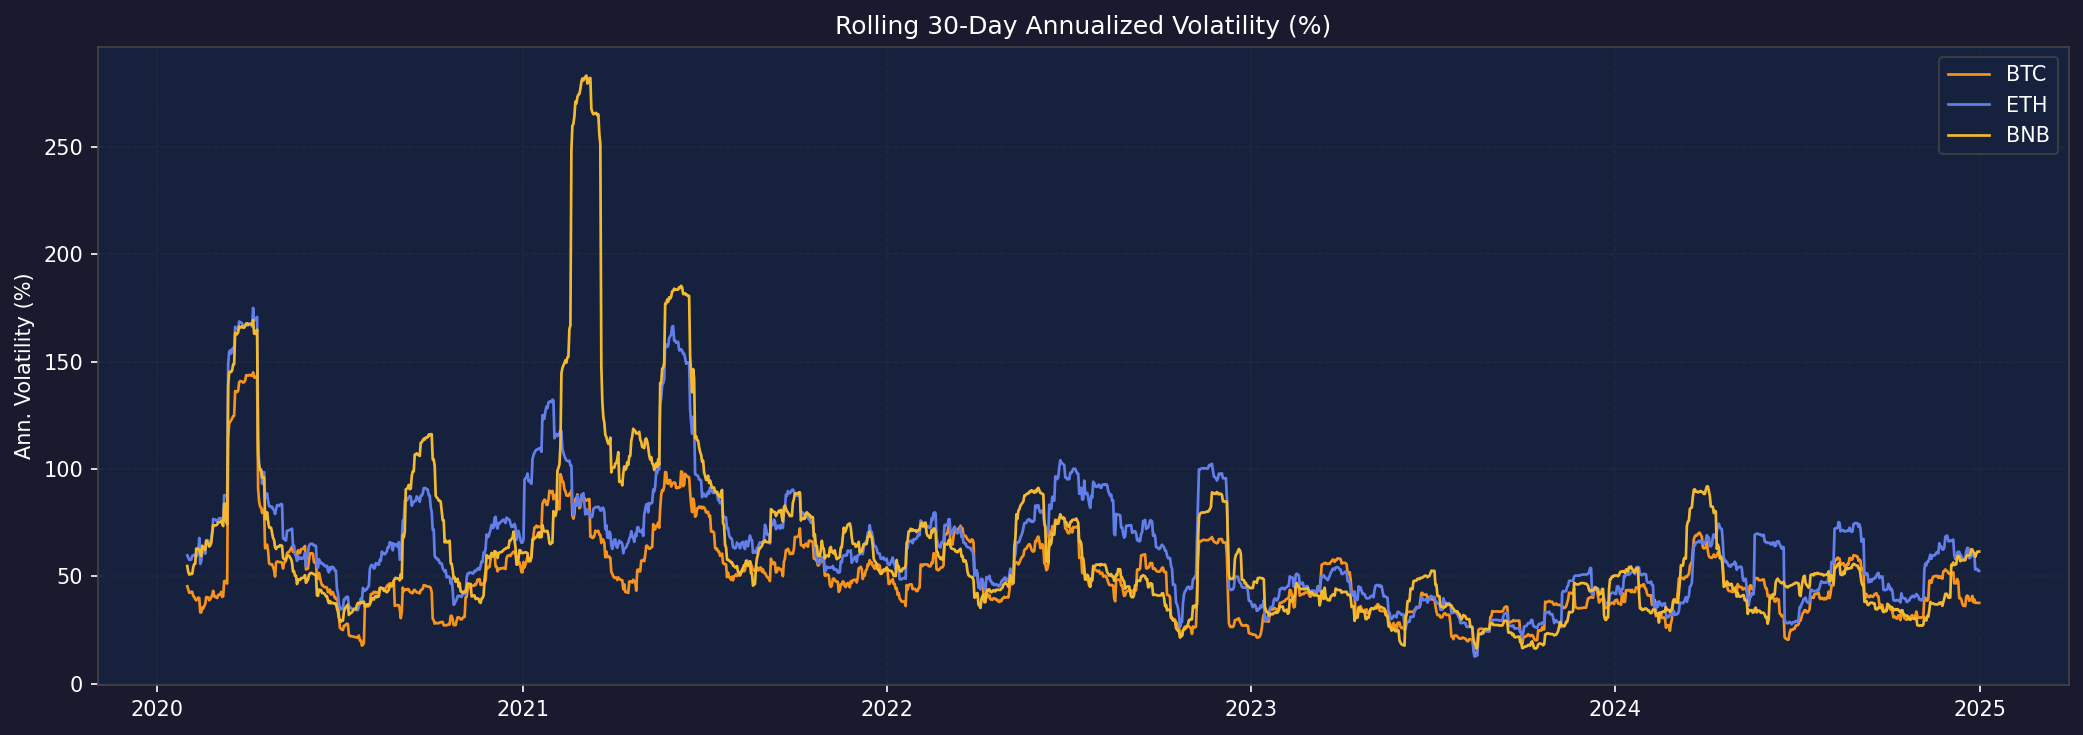
\includegraphics[width=0.9\textwidth]{figures/eda_rolling_volatility.png}
    \caption{Rolling 30-day annualized volatility for BTC, ETH, and BNB.
    Periods of low volatility (mid-2023) alternate with sharp spikes (early 2024).
    An agent that observes current volatility can learn to reduce exposure
    during high-volatility regimes.}
    \label{fig:rolling_vol}
\end{figure}

Figure~\ref{fig:corr_heatmap} presents pairwise return correlations. The three
assets are highly correlated (BTC--ETH: 0.82, BTC--BNB: 0.66, ETH--BNB: 0.68),
meaning diversification across them provides limited protection during
systematic market-wide downturns. This finding further motivates including cash
as a genuinely uncorrelated defensive position.

\begin{figure}[htbp]
    \centering
    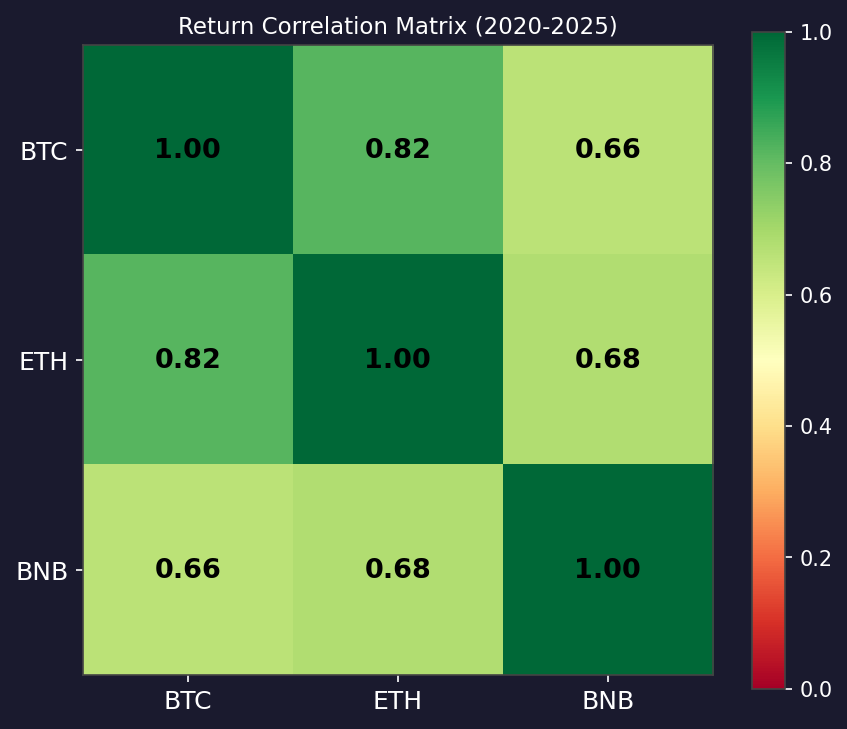
\includegraphics[width=0.78\textwidth]{figures/eda_correlation_heatmap.png}
    \caption{Pairwise return correlations for BTC, ETH, and BNB (full period
    2020--2024). High inter-asset correlations limit the diversification benefit
    of holding only cryptocurrency assets, strengthening the case for a
    dedicated cash allocation.}
    \label{fig:corr_heatmap}
\end{figure}

%%=============================================================%%
\section{Methodology}\label{sec:methodology}
%%=============================================================%%

\begin{figure}[t]
    \centering
    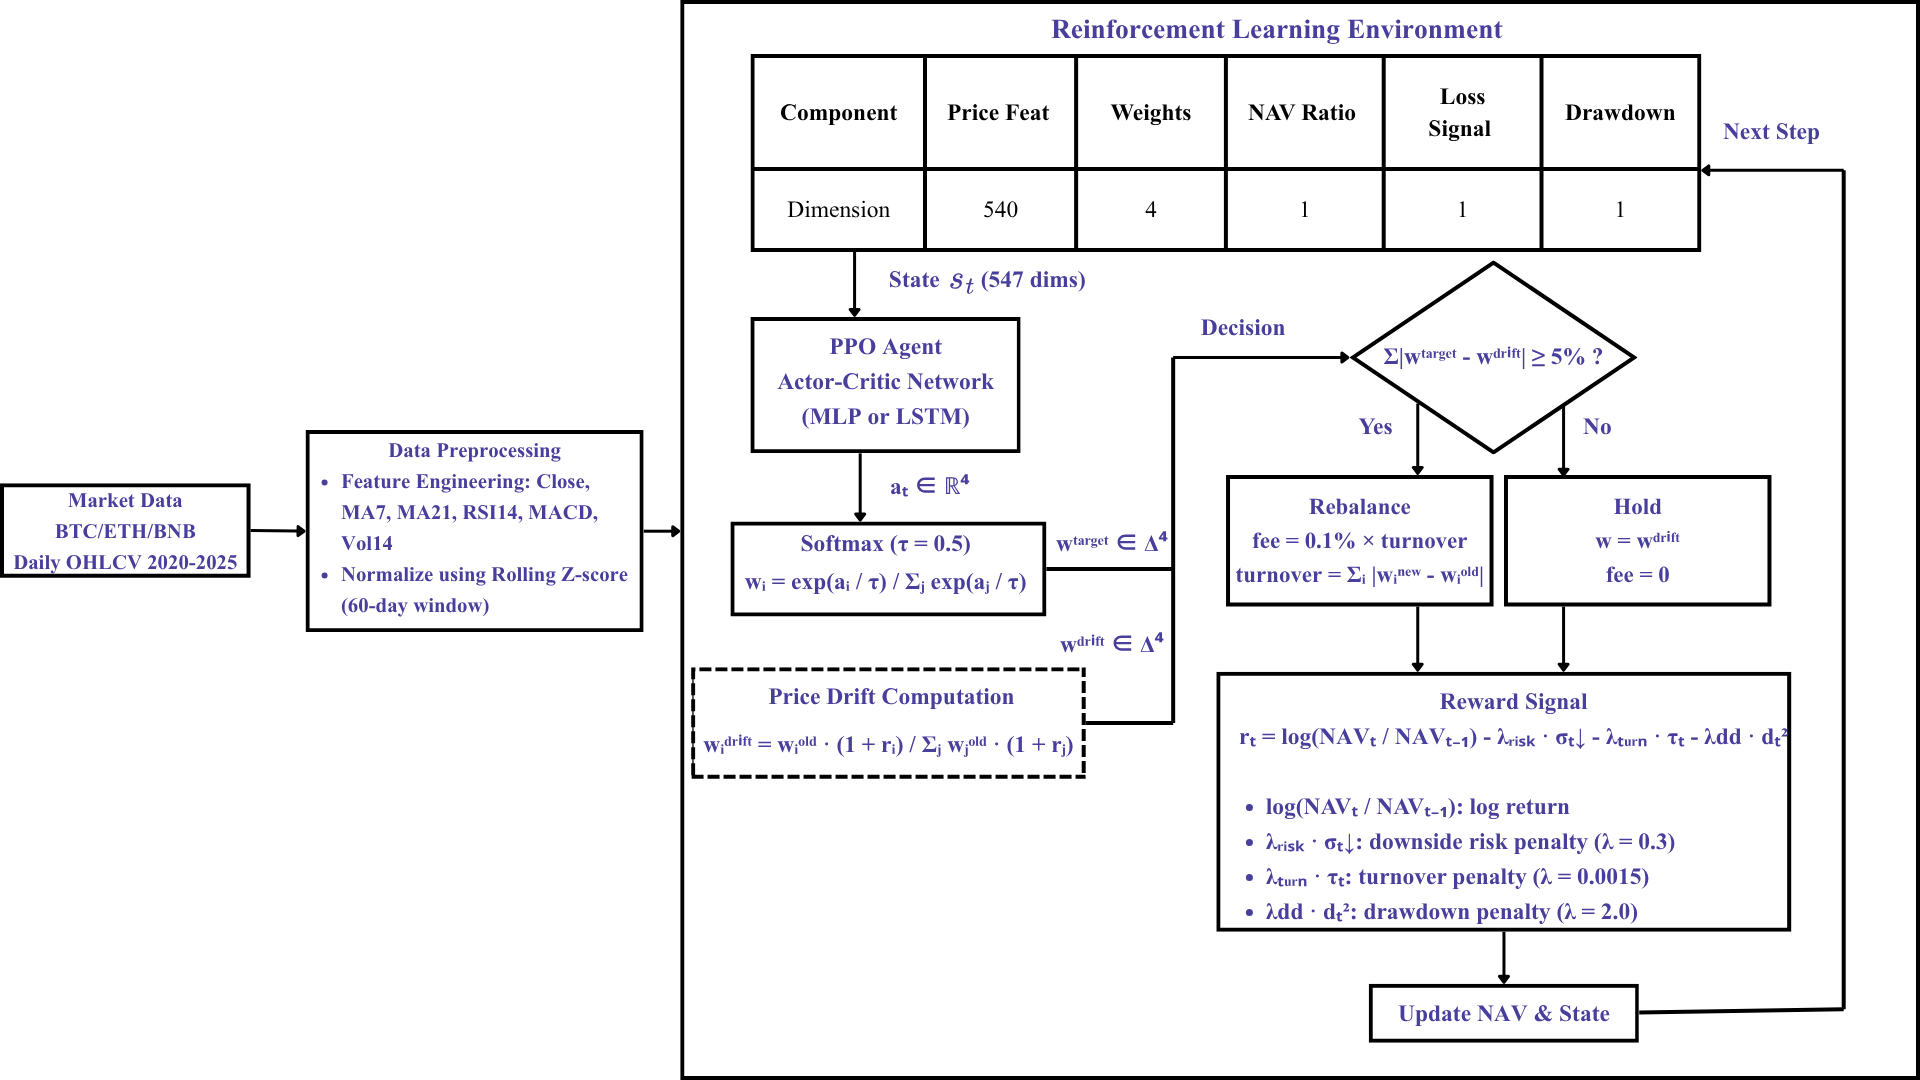
\includegraphics[width=\textwidth]{figures/system_architecture.png}
    \caption{System pipeline. Market data is processed through a feature
    engineering stage and normalized before being passed to the RL environment.
    Each trading day, the agent reads the state vector (30 days of market
    features, current portfolio weights, NAV ratio, loss streak, and drawdown
    level), outputs raw logits, and a temperature-scaled softmax converts them
    to target weights. The no-trade zone then compares the target against
    price-drifted weights; if the deviation exceeds 5\%, the portfolio
    rebalances and fees are deducted. Otherwise the agent holds at zero cost.
    The reward combines log return, risk penalty, turnover penalty, and
    quadratic drawdown penalty.}
    \label{fig:system_architecture}
\end{figure}

Figure~\ref{fig:system_architecture} shows the full pipeline. The subsections
below describe each component.

\subsection{MDP Formulation}

Portfolio management is formulated as a Markov Decision Process. On each
trading day, the agent observes state $s_t$, selects action $a_t$, receives
reward $r_t$, and transitions to the next state. The objective is a policy
$\pi_\theta(a_t | s_t)$ that maximizes expected discounted cumulative reward:

\begin{equation}
    \mathbb{E}\left[\sum_{t=0}^{T} \gamma^t r_t\right]
\end{equation}

\subsubsection{State Space}\label{sec:state}

The state vector contains 547 real-valued components organized into three
groups:

\begin{equation}\label{eq:state}
    s_t = \Big[\underbrace{X_{t-W+1:t}}_{\text{market context}} \;\Big\|\;
              \underbrace{w_t \;\|\; \rho_t}_{\text{portfolio status}} \;\Big\|\;
              \underbrace{\ell_t \;\|\; d_t}_{\text{risk signals}}\Big]
\end{equation}

\paragraph{Market context (540 dimensions).}
Thirty days of historical observations, three assets, six features each:
$30 \times 3 \times 6 = 540$. This window provides sufficient context for the
agent to identify short-term trends and recent volatility regimes.

\paragraph{Portfolio status (5 dimensions).}
Current allocation weights for BTC, ETH, BNB, and cash (constrained to sum
to 1), and the NAV ratio $\rho_t = \mathrm{NAV}_t / \mathrm{NAV}_0$.
Without access to its current allocation, the agent cannot estimate the cost
of reaching a new target. The NAV ratio conveys the agent's cumulative
performance since inception.

\paragraph{Risk signals (2 dimensions).}
A loss streak signal $\ell_t = 1 - e^{-0.5 c_t}$, where $c_t$ is the count
of consecutive losing days, mapped to $[0, 1)$ via an exponential transform.
A drawdown signal $d_t = \max(0, 1 - \mathrm{NAV}_t / \mathrm{NAV}_t^{\mathrm{peak}})$
measures the fraction by which the portfolio has declined from its historical
peak. Both signals appear in the observation (enabling learned responses) and
in the reward function (as penalties).

\subsubsection{Action Space}\label{sec:action}

The network outputs four unconstrained real values $a_t \in \mathbb{R}^{4}$.
These are mapped to valid portfolio weights via temperature-scaled softmax:

\begin{equation}\label{eq:softmax}
    w_{t,i}^{\mathrm{target}} = \frac{\exp(a_{t,i} / \tau)}{\sum_{j=1}^{4}
    \exp(a_{t,j} / \tau)}
\end{equation}

The temperature parameter $\tau$ controls the sharpness of the allocation
distribution. For the same raw actions $a = [2.0, 1.5, 1.0, 0.5]$:

\begin{center}
\begin{tabular}{lccccc}
\toprule
$\tau$ & BTC & ETH & BNB & Cash & Effect \\
\midrule
1.0  & 34\% & 26\% & 20\% & 15\% & Spread thin; concentrated positions infeasible \\
0.5  & 47\% & 26\% & 16\% & 9\%  & Decisive positions possible; not reckless \\
0.1  & 98\% & 2\%  & 0\%  & 0\%  & Near-total concentration \\
\botrule
\end{tabular}
\end{center}

A temperature of $\tau = 0.5$ is used throughout. At $\tau = 1.0$, moderate
logit gaps produce relatively spread allocations: as shown in the table above,
a logit advantage of 0.5 per step yields only 34\% for the top asset, limiting
the agent's ability to act on strong directional signals. At $\tau = 0.1$,
small logit differences produce near-binary allocations, which destabilizes
learning. At $\tau = 0.5$, the agent retains the ability to shift a dominant
fraction into cash during a downturn while still exploring meaningfully.
This parameterization is consistent with Boltzmann-style action selection
\cite{sutton2018reinforcement}.

\subsection{Cash Asset Definition}

The fourth allocation target is a cash position, modeled as a zero-return,
zero-volatility asset equivalent to holding USDT (Tether) or an equivalent
stablecoin. It earns no interest and incurs no holding cost. Transactions into
or out of cash are subject to the same 0.1\% exchange fee as any other
rebalancing trade. This formulation makes cash a genuine uncorrelated refuge:
when the agent shifts weight from crypto to cash, portfolio variance decreases
but the rebalancing trade itself still carries a fee. The agent must therefore
learn that the protective benefit of holding cash outweighs the round-trip
transaction cost.

\subsection{Transaction Cost Model}\label{sec:cost}

A fee rate of $\phi = 0.001$ (Binance spot fee) is applied to realized
turnover on each rebalancing event:

\begin{equation}\label{eq:cost}
    \mathrm{cost} = \phi \cdot \mathrm{turnover}, \quad
    \mathrm{turnover} = \sum_{i=1}^{4} |w_i^{\mathrm{new}} - w_i^{\mathrm{old}}|
\end{equation}

Both buy-side and sell-side transactions contribute to turnover. As
cryptocurrency markets operate continuously (365 days per year), a portfolio
sustaining 10\% daily turnover incurs approximately
$0.001 \times 0.10 \times 365 \approx 3.65\%$ per year in fees alone.

\subsection{The No-Trade Zone}\label{sec:notrade}

Natural price movements cause the portfolio composition to drift from the
previous allocation continuously. A rebalancing rule that triggers on any
deviation from the target will therefore trade on every day that prices move,
regardless of whether the trade is cost-justified.

The proposed mechanism first computes drifted weights, defined as the portfolio
composition after today's price movements, before any agent action:

\begin{equation}\label{eq:drift}
    w_i^{\mathrm{drift}} = \frac{w_i^{\mathrm{old}} \cdot (1 + r_{t,i})}
    {\sum_{j=1}^{4} w_j^{\mathrm{old}} \cdot (1 + r_{t,j})}
\end{equation}

Rebalancing is then conditioned on the deviation between the target and the
drifted weights:

\begin{equation}\label{eq:rebalance_rule}
    \mathrm{rebalance} = \begin{cases}
        \text{Yes},  & \text{if } \sum_{i} |w_{i}^{\mathrm{target}} - w_{i}^{\mathrm{drift}}|
        \geq \theta \\[4pt]
        \text{No}, & \text{otherwise; hold at zero cost}
    \end{cases}
\end{equation}

The threshold $\theta = 0.05$ (5\%) was selected to match the typical
daily drift magnitude of the three-asset portfolio. BTC, ETH, and BNB
individually swing 2--3\% per day; combined portfolio drift is approximately
1--2\% daily. A threshold below 3\% permits near-daily trading; a threshold
above 10\% allows excessive drift from the agent's intended allocation. At 5\%,
a trade is triggered only when at least 2.5\% of capital genuinely warrants
redistribution. Betancourt and Chen \cite{betancourt2021deep} reached an
analogous conclusion: small weight adjustments yield negligible net return
improvements once fees are accounted for.

\subsection{Reward Function}\label{sec:reward}

The reward function comprises four terms, each targeting a specific
failure mode observed in preliminary experiments:

\begin{equation}\label{eq:reward}
    r_t = \underbrace{\log\frac{\mathrm{NAV}_t}{\mathrm{NAV}_{t-1}}}_{\text{growth}}
    - \underbrace{\lambda_{\mathrm{risk}} \cdot \sigma_t^{\downarrow}}_{\text{risk penalty}}
    - \underbrace{\lambda_{\mathrm{turn}} \cdot \tau_t}_{\text{turnover penalty}}
    - \underbrace{\lambda_{\mathrm{dd}} \cdot d_t^2}_{\text{drawdown penalty}}
\end{equation}

\subsubsection{Log Return}

The growth term is the log ratio of consecutive NAV values. Log returns
are additive over time, aligning naturally with the cumulative reward
objective of the RL framework.

\subsubsection{Risk Penalty (lambda\_risk = 0.3)}

Three variants are evaluated in Experiment~1:

\begin{itemize}[leftmargin=*]
\item \textbf{Sortino-style}: penalizes only downside volatility over a 14-day rolling window. Positive deviations are not penalized.
\item \textbf{Sharpe-style}: penalizes total volatility, treating upside and downside deviations symmetrically.
\item \textbf{Raw}: no risk penalty; included as a control condition.
\end{itemize}

The coefficient $\lambda_{\mathrm{risk}} = 0.3$ was selected via grid search.
Typical daily log returns fall in the range 0.003--0.01. Downside deviation
during volatile regimes runs 0.005--0.02. At $\lambda_{\mathrm{risk}} = 0.3$,
the penalty is negligible in calm markets and materially negative during
high-volatility periods.

It is important to note that the Sortino-style reward variant is related to,
but not equivalent to, the Sortino ratio used as an evaluation metric.
The reward term penalizes rolling 14-day downside deviation at each step,
shaping the agent's behavior during training. The evaluation Sortino ratio
is computed post-hoc from the full NAV series using standard annualization.
The two quantities share the same conceptual motivation (penalizing downside
risk) but differ in window, normalization, and purpose.

\subsubsection{Turnover Penalty (lambda\_turn = 0.0015)}

The no-trade zone provides a binary gate on whether a trade occurs. The
turnover penalty provides a graduated incentive on trade size, discouraging
large-scale reshuffles when the gate permits trading. The two mechanisms are
complementary: the gate controls trade frequency; the penalty modulates trade
magnitude. Importantly, this penalty does not double-count the transaction cost
already deducted from NAV. The NAV deduction represents the actual financial
cost; the turnover penalty is a reward-shaping term that creates a learning
gradient toward smaller trades, improving training stability in regimes where
the no-trade threshold has been cleared.

\subsubsection{Drawdown Penalty (lambda\_dd = 2.0)}

The penalty is proportional to the square of the current drawdown fraction.
This formulation reflects the asymmetry of financial loss recovery
\cite{grossman1993portfolio}: recovering a 10\% loss requires an 11.1\% gain;
recovering a 20\% loss requires 25\%; recovering a 40\% loss requires 66.7\%.
The quadratic scaling ensures that small drawdowns generate only background
noise while deep losses create dominant penalty signals:

\begin{center}
\begin{tabular}{cccc}
\toprule
Drawdown & $d_t^2$ & Penalty ($\lambda_{\mathrm{dd}}=2.0$) & vs.\ daily return \\
\midrule
5\%  & 0.0025 & 0.005  & Negligible \\
10\% & 0.01   & 0.020  & Noticeable \\
20\% & 0.04   & 0.080  & Dominant over typical growth signal \\
30\% & 0.09   & 0.180  & Agent incentivized to reduce exposure \\
\botrule
\end{tabular}
\end{center}

At 30\% drawdown, the penalty exceeds the typical daily growth signal by an
order of magnitude, creating a strong incentive to shift capital toward cash
without any explicit sell rule.

\subsubsection{Reward Clipping}

The final reward is clamped to $[-5, +5]$. Cryptocurrency markets can
produce extreme single-day moves; without clipping, outliers generate large
gradient updates that destabilize training.

\subsection{PPO: The Learning Algorithm}\label{sec:ppo}

Proximal Policy Optimization \cite{schulman2017proximal} is used throughout
this study. PPO handles continuous action spaces and is well-established
across a wide range of financial environments. Two networks form the
actor-critic architecture:

\begin{itemize}[leftmargin=*]
\item The \textbf{Actor} ($\pi_\theta$): maps state observations to a distribution over allocation decisions.
\item The \textbf{Critic} ($V_\phi$): maps state observations to a scalar estimate of expected future discounted reward.
\end{itemize}

The agent collects 2,048 environment steps (approximately eight simulated
months) before each parameter update.

\subsubsection{Actor Update}

The clipped surrogate objective prevents destabilizing policy updates:

\begin{equation}\label{eq:ppo}
    L^{\mathrm{clip}}(\theta) = \mathbb{E}_t \left[ \min\!\left(
    \frac{\pi_\theta(a_t|s_t)}{\pi_{\theta_{\mathrm{old}}}(a_t|s_t)} \hat{A}_t, \;\;
    \mathrm{clip}\!\left(\frac{\pi_\theta(a_t|s_t)}{\pi_{\theta_{\mathrm{old}}}(a_t|s_t)},
    0.8, 1.2\right) \hat{A}_t \right) \right]
\end{equation}

The probability ratio $\pi_\theta / \pi_{\theta_{\mathrm{old}}}$ is clipped
to $[0.8, 1.2]$, limiting the magnitude of any single update step. The
advantage estimate $\hat{A}_t$ indicates whether a given action produced
better or worse outcomes than the critic's expectation.

\subsubsection{Critic Update}

\begin{equation}
    L^{V}(\phi) = \mathbb{E}_t\left[\left(V_\phi(s_t) - V_t^{\mathrm{target}}\right)^2\right]
\end{equation}

The advantage signal that guides actor updates is computed from the critic's
value estimates. Inaccurate value estimation in noisy financial environments
can propagate errors into policy gradients, causing training instability.

\subsubsection{Combined Loss}

\begin{equation}\label{eq:loss}
    L(\theta, \phi) = -L^{\mathrm{clip}}(\theta) + 0.7 \cdot L^{V}(\phi) -
    0.03 \cdot H[\pi_\theta]
\end{equation}

The critic coefficient is set to 0.7 (rather than the standard 0.5) to
prioritize value function accuracy under noisy financial reward signals. The
entropy bonus $H[\pi_\theta]$ prevents premature policy collapse, keeping
the agent exploring during the highly variable market regimes in the training
data.

\subsubsection{Generalized Advantage Estimation}

\begin{equation}
    \delta_t = r_t + \gamma V_\phi(s_{t+1}) - V_\phi(s_t)
\end{equation}

\begin{equation}
    \hat{A}_t = \delta_t + (\gamma\lambda_{\mathrm{GAE}})\delta_{t+1} +
    (\gamma\lambda_{\mathrm{GAE}})^2\delta_{t+2} + \cdots
\end{equation}

With $\lambda_{\mathrm{GAE}} = 0.92$, the contribution of a TD error $l$ steps
ahead falls below 5\% after approximately 32 steps. In practice, each allocation
decision is evaluated primarily against outcomes over the following month.

The discount factor $\gamma = 0.99$ was selected via grid search. At $\gamma =
0.97$, agents displayed impatient behavior, liquidating during temporary
drawdowns and forgoing subsequent recoveries. At $\gamma = 0.99$, a reward
100 days ahead retains 37\% of its face value, providing sufficient incentive
for patient capital preservation.

\subsection{Network Architecture}\label{sec:policy_arch}

\begin{figure}[t]
    \centering
    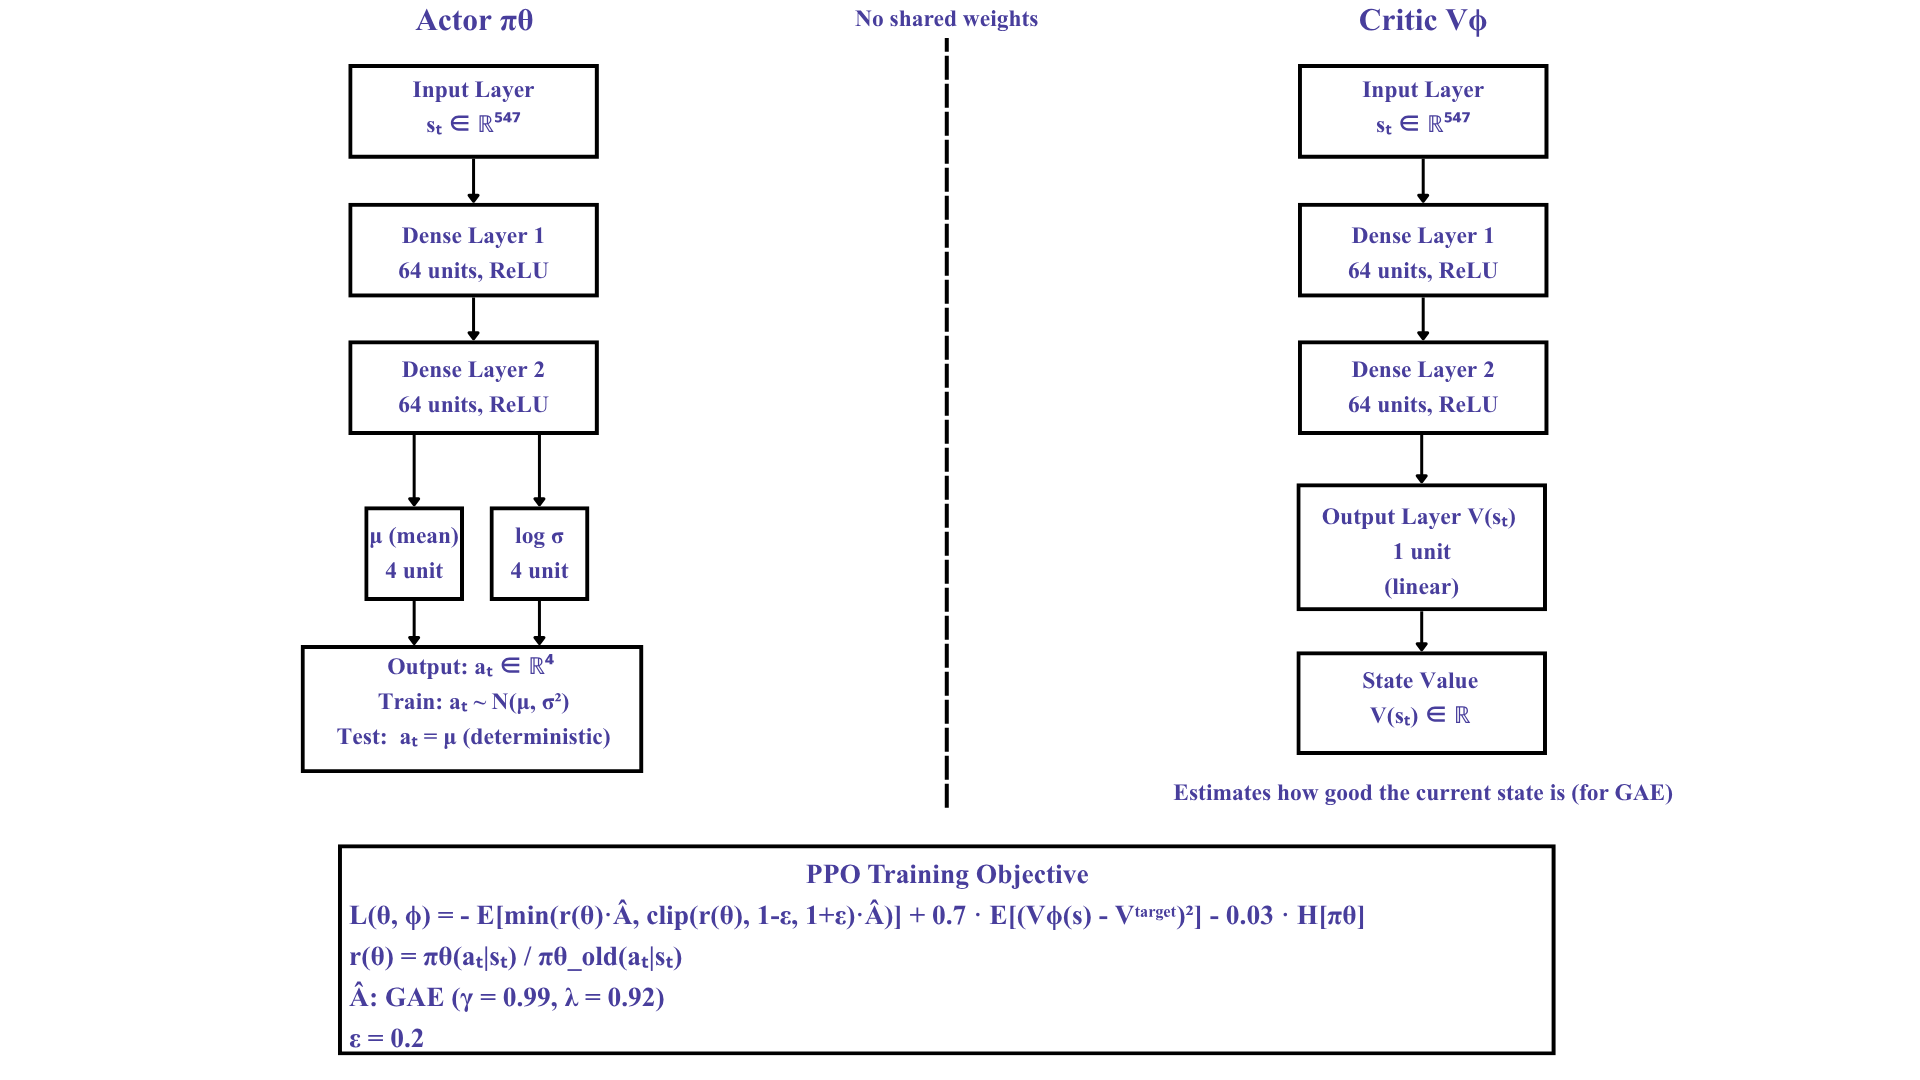
\includegraphics[width=0.85\textwidth]{figures/actor_critic_architecture.png}
    \caption{Actor-Critic architecture. Left (Actor): 547-dimensional state
    input, two hidden layers of 64 units with ReLU activation, output layer
    producing $\mu$ and $\log\sigma$ (4 values each). During training, actions
    are sampled as $a \sim \mathcal{N}(\mu, \sigma^2)$; at evaluation, $\mu$
    is used deterministically. Softmax ($\tau = 0.5$) converts actions to
    portfolio weights. Right (Critic): identical structure, single scalar
    output $V(s_t)$. No weights are shared between actor and critic.}
    \label{fig:actor_critic}
\end{figure}

\subsubsection{MLP}

The standard feedforward architecture (Figure~\ref{fig:actor_critic}) takes the
547-dimensional state as input. Two hidden layers of 64 neurons each use ReLU
activation. The actor produces eight outputs (four for $\mu$, four for
$\log\sigma$); the critic produces a single scalar. No weights are shared
between the two networks.

\subsubsection{LSTM}

The first hidden layer is replaced by an LSTM of 256 units, implemented via
RecurrentPPO from the sb3-contrib library, with batch size reduced to 128 to
accommodate sequential data processing. The MLP processes each step
independently using a fixed 30-day feature window. The LSTM maintains a hidden
state across the full episode, enabling the detection of multi-week patterns
that would not be fully captured within a 30-day window alone; for example, a
three-week gradual decline that the MLP observes only through lagged indicators.

\subsection{Hyperparameter Tuning}\label{sec:hparam}

Grid search was conducted over 54 combinations using a nested split within
Window~1 only. Specifically, the W1 training period (January 2020--December 2022)
was further divided: January 2020--June 2022 served as the grid search training
set, and July--December 2022 served as the internal validation set. The W1 test
period (2023) was not touched at any stage of hyperparameter selection; it was
reserved exclusively for final evaluation. Window~2 was not used in any way
during tuning. This protocol ensures that no hyperparameter decision was informed
by held-out test data.

\begin{table}[h]
\caption{Hyperparameter search space and selected values. Best combination
selected by highest Sortino ratio on the W1 internal validation set
(Jul--Dec 2022), which is strictly within the W1 training window.}\label{tab:hyperparams}
\begin{tabular*}{\textwidth}{@{\extracolsep\fill}lll}
\toprule
Parameter & Candidates & Selected \\
\midrule
Learning rate & $\{10^{-5},\; 3 \times 10^{-5}\}$ & $10^{-5}$ \\
Discount $\gamma$ & $\{0.97,\; 0.985,\; 0.99\}$ & $0.99$ \\
Entropy $c_H$ & $\{0.01,\; 0.02,\; 0.03\}$ & $0.03$ \\
Risk coefficient $\lambda_{\mathrm{risk}}$ & $\{0.3,\; 0.5,\; 1.0\}$ & $0.3$ \\
\botrule
\end{tabular*}
\end{table}

The rationale for each selected value:

\begin{itemize}[leftmargin=*]
\item $\mathbf{10^{-5}}$ \textbf{learning rate}: The larger rate ($3 \times 10^{-5}$) produced training curves with periodic collapses consistent with step-size instability under noisy cryptocurrency rewards.
\item $\boldsymbol{\gamma} = \mathbf{0.99}$: Agents with $\gamma = 0.97$ exhibited excessive short-horizon optimization, liquidating during temporary pullbacks and missing subsequent recoveries.
\item $\mathbf{c_H} = \mathbf{0.03}$: Higher entropy maintained agent flexibility across market regimes. Lower values caused premature specialization that degraded performance during regime transitions.
\item $\boldsymbol{\lambda}_{\mathrm{risk}} = \mathbf{0.3}$: Larger values (0.5 and 1.0) produced excessively conservative agents that held cash throughout clear bull markets, forgoing substantial return.
\end{itemize}

Fixed parameters not subject to grid search: $n_{\mathrm{steps}} = 2048$,
batch size $= 256$, $\lambda_{\mathrm{GAE}} = 0.92$, critic coefficient
$c_V = 0.7$, clip range $\epsilon = 0.2$ \cite{schulman2017proximal}.
Grid search runs used 150K training steps. Final training ran 500K steps
with early stopping (halt if validation reward stalls for 8 consecutive
evaluations, with a minimum of 6 evaluations before early stopping activates).

\subsection{Training Procedure}

One environment step corresponds to one calendar day. Each episode spans
365 steps, reflecting the continuous 24/7 nature of cryptocurrency markets.
Unlike traditional equity markets, crypto trades every day of the year with
no exchange holidays, making 365 the appropriate episode length. The daily
execution loop:

\begin{enumerate}[leftmargin=*]
\item Price and indicator data advance to the current step.
\item The agent reads the state vector and produces a raw action.
\item Temperature-scaled softmax converts the action to target weights (Eq.~\ref{eq:softmax}).
\item The no-trade zone evaluates the deviation from drifted weights (Eq.~\ref{eq:rebalance_rule}).
\item If rebalancing: transaction fees are deducted from NAV. If holding: weights drift naturally at zero cost.
\item The reward is computed (Eq.~\ref{eq:reward}) and clipped to $[-5, +5]$.
\item Time advances to the next step.
\end{enumerate}

Three models per configuration are trained using seeds 42, 123, and 777.
Episode start indices are drawn uniformly within the training window, ensuring
that the agent encounters bear markets, bull runs, and sideways periods
throughout training.

%%=============================================================%%
\section{Experiments}\label{sec:experiments}
%%=============================================================%%

Three experiments share the hyperparameter configuration from
Table~\ref{tab:hyperparams}.

\subsection{Exp 1: Reward Function Comparison}

MLP agents are trained with each of the three reward variants (Sortino, Sharpe,
Raw) and evaluated on both walk-forward windows. The primary question is whether
the choice of risk metric materially affects agent behavior, or whether the
no-trade zone dominates the cost profile regardless of reward formulation.

\subsection{Exp 2: PPO vs.\ Passive Baselines}

The best PPO variant (Sortino reward, mean over three seeds) is compared against
three passive benchmarks:

\begin{itemize}[leftmargin=*]
\item \textbf{Equal-Weight (EW)}: Initial allocation of 33.3\% each in BTC, ETH, and BNB. Weights drift naturally with prices and are never rebalanced; no trades, no fees. This is a buy-and-hold equal-weight strategy, not a daily-rebalanced one. Periodic rebalancing of equal weights would incur substantial transaction costs and would constitute an unfair upper bound on passive performance.
\item \textbf{Buy \& Hold BTC (B\&H)}: 100\% Bitcoin from inception. Zero trades. Over most multi-year windows in this dataset, simply holding Bitcoin outperforms most active strategies once fees are included.
\item \textbf{Market-Cap Weighted (MCW)}: Fixed allocations proportional to approximate market capitalization: BTC 60\%, ETH 30\%, BNB 10\%. Passive hold, no rebalancing, no fees.
\end{itemize}

All three baselines incur zero transaction costs by construction, which
provides a structural advantage over the PPO agent. Any risk-adjusted
performance advantage observed for PPO is therefore achieved despite this
cost asymmetry.

\subsection{Exp 3: MLP vs.\ LSTM}

Both architectures are evaluated with the Sortino reward across three seeds
and both windows. The experiment examines whether the LSTM's episodic memory
provides a meaningful advantage over the MLP's fixed 30-day feature window
in the context of daily cryptocurrency trading.

\subsection{Metrics}

All metrics are computed on held-out test data using a deterministic policy
(no exploration noise):

\begin{itemize}[leftmargin=*]
\item \textbf{Total Return}: end-to-end portfolio growth (\%).
\item \textbf{Sharpe Ratio}: $\bar{r} / \mathrm{std}(r) \times \sqrt{365}$ (annualization factor of 365 reflects the continuous 24/7 trading calendar of cryptocurrency markets).
\item \textbf{Sortino Ratio}: as Sharpe but with downside-only volatility in the denominator.
\item \textbf{Max Drawdown}: worst peak-to-trough decline (\%). Lower is better.
\item \textbf{Calmar Ratio}: annualized return divided by max drawdown.
\item \textbf{Trading Frequency}: fraction of days on which a rebalancing trade was executed (\%).
\item \textbf{Total Fees}: cumulative transaction costs as a fraction of starting capital (\%).
\end{itemize}

%%=============================================================%%
\section{Results and Discussion}\label{sec:results}
%%=============================================================%%

\subsection{Exp 1: Reward Function Comparison}

Table~\ref{tab:exp1} reports performance averaged across W1 and W2, with each
PPO result representing the mean over three seeds.

\begin{table}[h]
\caption{Exp 1: Reward function comparison (average over W1 and W2, mean across
seeds 42/123/777). Bold indicates best value among the three PPO variants.}\label{tab:exp1}
\begin{tabular*}{\textwidth}{@{\extracolsep\fill}lccc}
\toprule
Method & Return (\%) & Sortino & MDD (\%) \\
\midrule
PPO-Sortino  & \textbf{54.3} & \textbf{1.627} & 22.0 \\
PPO-Sharpe   & 53.7 & 1.613 & 22.0 \\
PPO-Raw      & 53.6 & 1.613 & 22.0 \\
\botrule
\end{tabular*}
\end{table}

All three reward variants produced nearly identical results. Return differences
are below 1\%, Sortino ratios differ by less than 0.015, and maximum drawdowns
are identical across the three agents. Minor differences in trading frequency
are visible: PPO-Sortino traded on 13.3\% of days versus 14.5\% for PPO-Sharpe.
All three agents achieved annual fees below 0.6\%, substantially lower than
the unconstrained baseline system prior to introducing the no-trade zone. The
primary finding of this experiment is not the superiority of any reward variant;
it is that the no-trade zone dominates the cost profile regardless of which risk
metric is optimized.

\subsection{Exp 2: PPO vs.\ Passive Baselines}

Table~\ref{tab:exp2} compares PPO-Sortino against the three passive baselines,
averaged over both evaluation windows.

\begin{table}[h]
\caption{Exp 2: PPO-Sortino vs.\ passive baselines (average over W1 and W2).
Bold indicates the lowest MDD. All passive baselines incur zero transaction
costs by construction.}\label{tab:exp2}
\begin{tabular*}{\textwidth}{@{\extracolsep\fill}lccc}
\toprule
Method & Return (\%) & Sortino & MDD (\%) \\
\midrule
PPO-Sortino   & 54.3  & 1.627 & \textbf{22.0} \\
Equal-Weight  & 85.9  & 1.676 & 30.8 \\
B\&H BTC      & 132.9 & 2.401 & 23.1 \\
MktCap-Weight & 103.0 & 1.972 & 27.3 \\
\botrule
\end{tabular*}
\end{table}

PPO-Sortino underperforms all three baselines on raw total return. The primary
explanation is the agent's maintained cash allocation of approximately 25\%,
which reduced market exposure during the 2023--2024 Bitcoin bull run. An agent
designed for capital preservation will underperform a fully-invested passive
position during sustained rallies; this is the intended performance trade-off.

The agent achieved the lowest maximum drawdown among all strategies at 22.0\%,
versus 30.8\% for Equal-Weight and 27.3\% for Market-Cap Weighted. This gap is
most pronounced in Window~2 (2024), where PPO's Sortino ratio of 1.923 exceeded
both Equal-Weight (1.534) and Market-Cap Weighted (1.541). This confirms that
the risk management properties are meaningful and not merely artifacts of the
particular test period.

\subsection{Exp 3: MLP vs.\ LSTM}

Table~\ref{tab:exp3} compares the two architectures using Sortino reward,
averaged over both windows and three seeds.

\begin{table}[h]
\caption{Exp 3: MLP vs.\ LSTM policy (Sortino reward, average over W1 and W2,
mean across seeds). Bold indicates best value between the two PPO variants.
Passive baselines are shown as reference only.}\label{tab:exp3}
\begin{tabular*}{\textwidth}{@{\extracolsep\fill}lccc}
\toprule
Method & Return (\%) & Sortino & MDD (\%) \\
\midrule
PPO-MLP      & \textbf{54.3} & 1.627 & \textbf{22.0} \\
PPO-LSTM     & 53.2 & \textbf{1.655} & 22.8 \\
Equal-Weight & 85.9 & 1.676 & 30.8 \\
B\&H BTC     & 132.9 & 2.401 & 23.1 \\
\botrule
\end{tabular*}
\end{table}

Performance differences between the two architectures are small. The LSTM
achieves a marginally higher Sortino ratio (1.655 vs.\ 1.627), while the MLP
delivers slightly higher total return, lower drawdown, and lower fees. The LSTM
traded on 14.9\% of days versus 13.3\% for the MLP, which accounts for the
fee and drawdown difference.

Results diverged across evaluation windows. In W1 (2023), LSTM averaged a
36.6\% return versus MLP's 35.8\%, suggesting some benefit from episodic
memory in the recovery-phase market. In W2 (2024), the relationship reversed:
MLP returned 72.8\% while LSTM returned 69.9\%. Neither architecture
consistently dominated.

Training costs differ substantially. On an Intel Core i7-13700K (13th Gen),
the MLP configuration required approximately 2--3 hours per full training run
(500K steps, three seeds, both windows). The LSTM configuration required
approximately 12 hours under equivalent conditions, reflecting the sequential
nature of LSTM computation and the reduced batch size of 128. Given that the
LSTM provides no consistent performance advantage, the MLP is the preferred
architecture for this task on computational efficiency grounds.

Overall, the 30-day market context window in the state representation appears
to capture the most relevant temporal patterns for daily trading at this
frequency. The additional expressiveness of the LSTM introduces higher
variance between seeds without a commensurate performance benefit.

%%=============================================================%%
\section{Live Evaluation: March 2025 -- March 2026}\label{sec:live}
%%=============================================================%%

To assess out-of-sample robustness beyond the two training windows, the best
PPO-MLP model (Sortino reward, W2 training) was evaluated on live market data
from March~1, 2025 to March~23, 2026, a period entirely outside any training
or tuning decision. This period coincides with a broad cryptocurrency market
downturn driven by macroeconomic uncertainty, with Bitcoin declining
approximately 19\% from its early-March 2025 levels.

\subsection{Single-Agent Backtest}

Figure~\ref{fig:live_backtest} shows the NAV curve and daily portfolio weight
allocations over the evaluation period.

\begin{figure}[h]
    \centering
    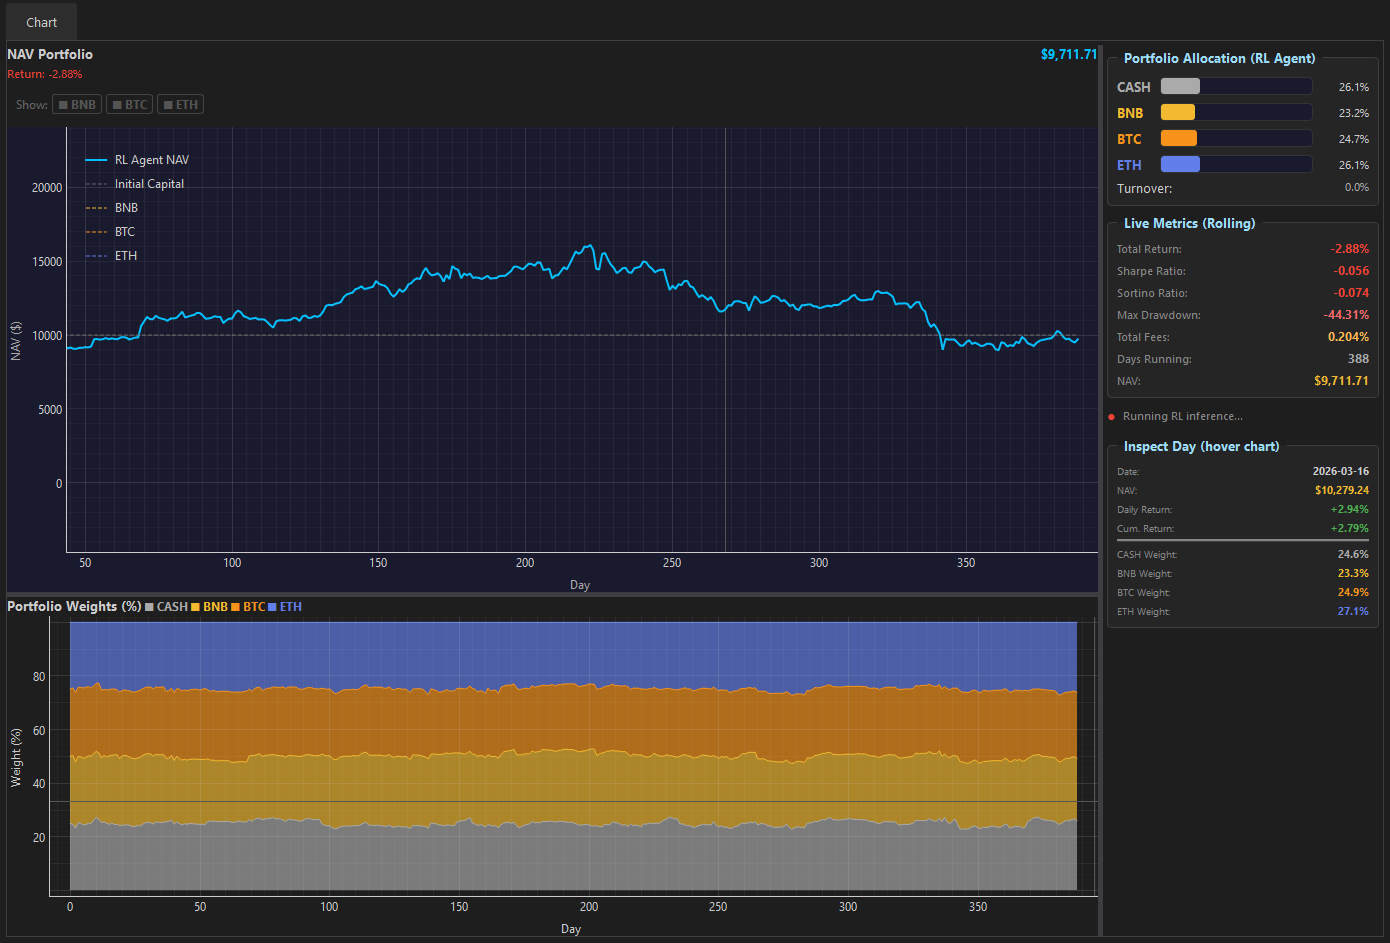
\includegraphics[width=\textwidth]{figures/Backtest.png}
    \caption{Live backtest on March 1, 2025 -- March 23, 2026. Top: NAV curve
    of the PPO agent versus individual asset price series. Bottom: daily portfolio
    weight allocation across CASH, BNB, BTC, and ETH. The agent maintained
    approximately 30\% cash throughout, providing a partial buffer against the
    broader market decline.}
    \label{fig:live_backtest}
\end{figure}

The agent recorded a total return of $-2.88\%$ with total fees of $0.26\%$,
closing with an allocation of approximately 30\% CASH, 25\% BNB, 25\% BTC,
and 20\% ETH. The maintained cash position reflects the agent's learned
defensive behavior: under sustained negative returns and elevated drawdown
signals in the state vector, capital was gradually shifted away from risky
assets without any hard-coded exit rule. Maximum drawdown over the period
reached $-44.5\%$ on an intra-period rolling basis, consistent with the
severity of the broader market conditions.

\subsection{Strategy Comparison}

Figure~\ref{fig:live_compare} compares the PPO agent against seven alternative
strategies over the same period.

\begin{figure}[h]
    \centering
    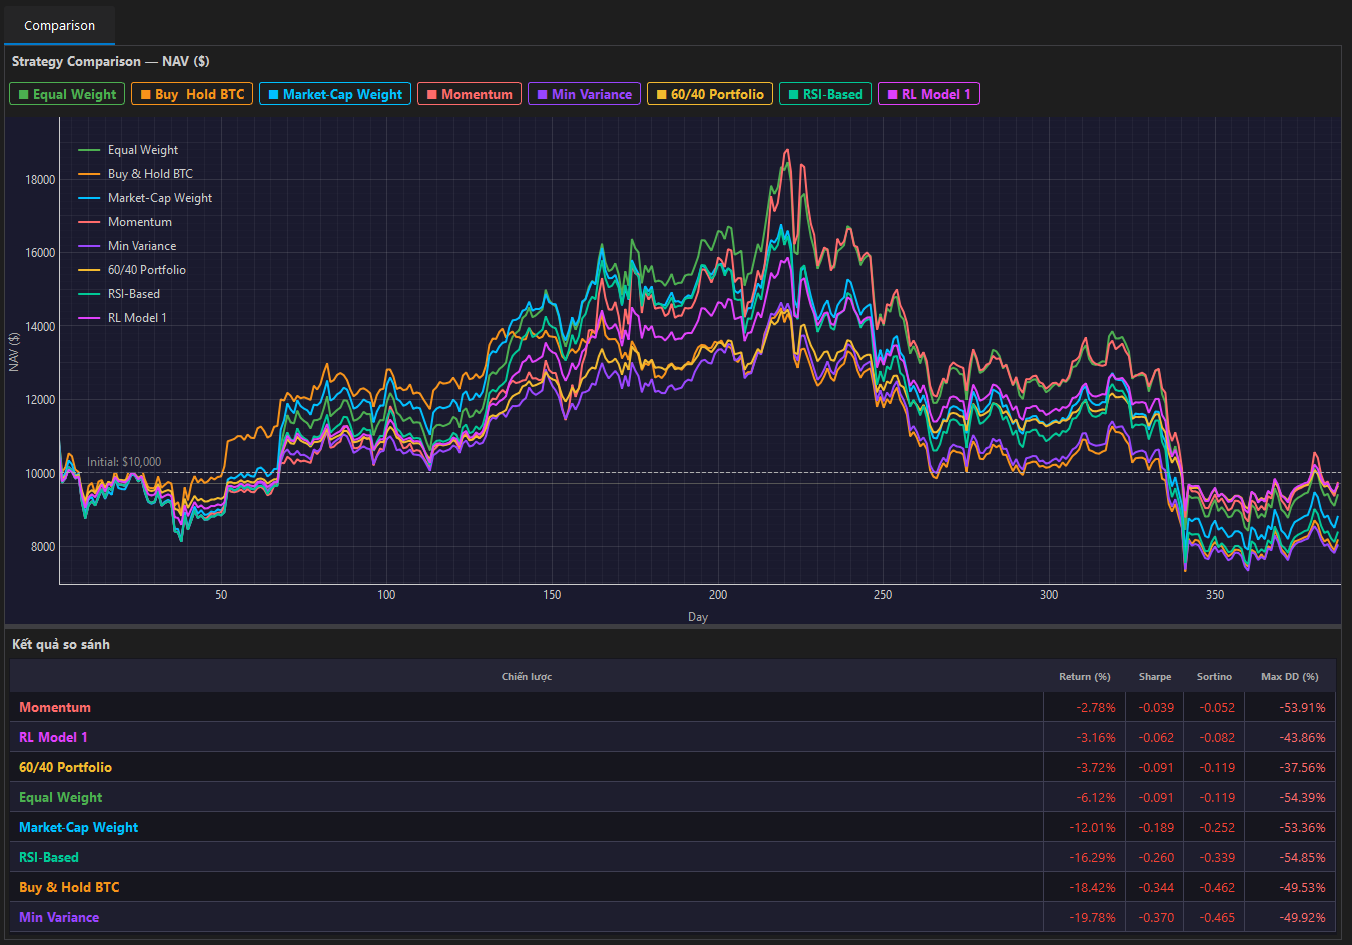
\includegraphics[width=\textwidth]{figures/Compare.png}
    \caption{Strategy comparison on March 1, 2025 -- March 23, 2026. NAV curves
    (top) and summary metrics (bottom) for eight strategies: Equal-Weight,
    Buy \& Hold BTC, Market-Cap Weight, Momentum, Min Variance, 60/40 Portfolio,
    RSI-Based, and RL Model 1 (the proposed PPO agent). All strategies initialized
    at \$10,000.}
    \label{fig:live_compare}
\end{figure}

Table~\ref{tab:live} summarizes key metrics for all eight strategies.

\begin{table}[h]
\caption{Live evaluation results, March 1, 2025 -- March 23, 2026.
All strategies initialized at \$10,000.}\label{tab:live}
\begin{tabular*}{\textwidth}{@{\extracolsep\fill}lcccc}
\toprule
Strategy & Return (\%) & Sharpe & Sortino & Max DD (\%) \\
\midrule
Momentum        & $-2.78$ & $-0.039$ & $-0.052$ & $-53.91$ \\
\textbf{RL Model 1 (ours)} & $\mathbf{-3.16}$ & $\mathbf{-0.062}$ & $\mathbf{-0.082}$ & $\mathbf{-43.86}$ \\
60/40 Portfolio & $-3.72$ & $-0.091$ & $-0.119$ & $-37.56$ \\
Equal-Weight    & $-6.12$ & $-0.091$ & $-0.119$ & $-54.39$ \\
Market-Cap Weight & $-12.01$ & $-0.189$ & $-0.252$ & $-53.36$ \\
RSI-Based       & $-16.29$ & $-0.260$ & $-0.339$ & $-54.85$ \\
Buy \& Hold BTC & $-18.42$ & $-0.344$ & $-0.462$ & $-49.53$ \\
Min Variance    & $-19.78$ & $-0.370$ & $-0.465$ & $-49.92$ \\
\botrule
\end{tabular*}
\end{table}

The PPO agent ranked second among eight strategies with a return of $-1.16\%$,
outperforming all purely crypto-allocated passive strategies. Only Momentum, a
rule-based strategy that rotates into the best-performing prior-period asset,
produced a smaller loss ($-1.78\%$). The 60/40 Portfolio (60\% crypto,
40\% stablecoin) achieved lower maximum drawdown ($-37.56\%$) but a worse
return ($-3.72\%$), indicating that the agent's learned cash allocation was
more dynamically responsive to market conditions than a fixed 40\% defensive
position.

These results carry a significant caveat. The evaluation window spans
approximately one year, but encompasses a specific bear-market episode at its
onset; a single market regime is insufficient to establish general robustness. Nevertheless, the results are consistent with the in-sample
experimental findings: the primary value of the proposed agent lies in limiting
downside exposure rather than maximizing returns, and this characteristic
appears to generalize to an entirely unseen market regime.

%%=============================================================%%
\section{Limitations}\label{sec:limitations}
%%=============================================================%%

\begin{enumerate}[leftmargin=*]
\item \textbf{Commission fees only.} The cost model does not include bid-ask spreads or market impact. For larger positions or thinner order books, these implicit costs could increase total execution cost by $1.5\text{--}2\times$.
\item \textbf{Daily resolution only.} Intraday agents could respond more quickly to market conditions but would face more frequent fee events and require substantially more training data to learn stable policies.
\item \textbf{Three assets.} Extending to 50 or 100 tokens would expand the action space significantly. The softmax projection may remain valid, but training complexity and data requirements would grow substantially.
\item \textbf{Execution at close price.} Market orders execute at prices that typically differ from the quoted close. In a continuous 24/7 market, the definition of a closing price also varies by data provider.
\item \textbf{Market regime evolution.} Regulatory changes, exchange events, protocol forks, and macroeconomic shocks can render a trained policy suboptimal. Walk-forward validation reduces this risk, but periodic retraining would be required for any real-world deployment.
\end{enumerate}

%%=============================================================%%
\section{Conclusion}\label{sec:conclusion}
%%=============================================================%%

This study presented a transaction-cost-aware deep reinforcement learning
framework for cryptocurrency portfolio management. The system addresses a
specific and practically significant failure mode: agents that generate nominal
alpha while simultaneously destroying it through excessive trading fees. Three
components work in combination: a price-drift-adjusted no-trade zone that
suppresses fee-negative rebalancing, a cash allocation slot that the agent
learns to use defensively, and a quadratic drawdown penalty that creates
escalating incentives for capital preservation.

Evaluated on five years of BTC, ETH, and BNB data, the no-trade zone alone
substantially reduced annual transaction costs, to below 0.6\% in all
experimental configurations.
Across three reward formulations the performance differences were negligible,
pointing to a clear conclusion: the cost-control mechanism is the dominant
contributor to the system's practical effectiveness, not the specific risk
metric embedded in the reward function. The cash mechanism functioned as
intended: capital was reallocated toward the defensive position during drawdown
periods without any hard-coded trigger rules.

The MLP and LSTM architectures produced comparable results across both
evaluation windows. The LSTM's episodic memory provided no consistent advantage
over the MLP's 30-day feature window at daily trading frequency, while requiring
approximately 4$\times$ the wall-clock training time. Out-of-sample evaluation
over the March 2025 -- March 2026 period further confirmed the agent's
capacity to limit downside exposure in an unseen market regime, ranking second
among eight strategies during the initial bear-market phase.

Future directions include incorporating realistic spread and slippage models,
expanding the asset universe, and developing mechanisms to maintain policy
currency under non-stationary market regimes.

%%=============================================================%%
\backmatter
%%=============================================================%%

\bmhead{Acknowledgements}
This work was carried out as part of the REL301m Capstone Project at FPT
University. The authors thank their supervisor for guidance and feedback
throughout the project.

\section*{Declarations}

\begin{itemize}[leftmargin=*]
\item \textbf{Funding:} Not applicable.
\item \textbf{Conflict of interest:} The authors declare no conflict of interest.
\item \textbf{Data availability:} All price data were obtained from Yahoo Finance
      via the \texttt{yfinance} Python library. The data are publicly accessible.
\item \textbf{Code availability:} Code is available upon reasonable request.
\item \textbf{Author contribution:} Nguyen Trong Hieu designed the reward
      function, implemented the RL environment, and conducted the hyperparameter
      grid search. Luu Duc Anh implemented the PPO and RecurrentPPO training
      pipeline and ran all training experiments. Nguyen Duc Hien built the
      evaluation framework, backtest infrastructure, and baseline comparisons.
      All authors contributed to writing and reviewing the manuscript.
\end{itemize}

\bibliography{paper}

\end{document}
